% ==============================================================================
% SECCION 6: ACTIVIDAD 5 - EFECTOS PARASITOS, FRECUENCIAS Y OPERACION NTV
% ==============================================================================
\section{Actividad 5: Efectos Parásitos, Ventana de Frecuencia y Operación en Tensión Reducida (NTV)}
\label{sec:actividad5}

En tecnologías submicrométricas profundas ($45\,\text{nm}$), el escalado de tensión hacia el régimen \textit{Near-Threshold Voltage} (NTV) y subumbral reduce drásticamente el consumo dinámico, pero exacerba los efectos parásitos de acoplamiento capacitivo y degrada los márgenes de retención frente a corrientes de fuga. Esta sección analiza el fenómeno de \textit{clock feedthrough} en el PMOS de precarga, determina experimentalmente los límites de frecuencia $[f_{\min}, f_{\max}]$ que confinan la ventana operable de la lógica dominó, contrasta los nodos PTM 45\,nm HP y LP en subumbral ($V_{DD} = 0.50\,\text{V}$) y cuantifica el escalado de energía por ciclo.

\subsection{Sobreimpulso por Clock Feedthrough, Recorte por Diodo y Amortiguamiento}
Se evaluó la respuesta transitoria del nodo dinámico durante la transición de precarga ($CLK: 1 \to 0$ con $t_r = t_f = 5\,\text{ps}$) en la compuerta NAND3 dinámica (PTM 45\,nm HP, $V_{DD} = 1.0\,\text{V}$, $C_L = 0.5\,\text{fF}$).

\begin{enumerate}[leftmargin=1.4em,itemsep=0.01em]
  \item \textbf{Mecanismo Físico y Modelo Analítico:} La capacitancia parásita compuerta-drenaje del PMOS ($W_p = 135\,\text{nm}$), $C_{gd} = (cgdo + cgdl)W_p \approx \mathbf{0.0507\,\text{fF}}$, forma un divisor capacitivo con el nodo ($C_{\text{total}} \approx 0.85\text{--}1.05\,\text{fF}$), prediciendo un sobreimpulso analítico de $\Delta V \approx V_{DD}\frac{C_{gd}}{C_{\text{total}}} \approx \mathbf{50\text{--}60\,\text{mV}}$.
  \item \textbf{Validación Experimental y Recorte Transitorio por Diodo $D_{DB}$:} Sin keeper, la simulación registra un sobreimpulso de $\mathbf{+64.31\,\text{mV}}$ ($V_{dyn,\max} = 1.0643\,\text{V}$, Figura~\ref{fig:feedthrough_energia}(a)), reproduciendo la cota experimental de referencia ($+61.30\,\text{mV}$, con desviación relativa inferior al $4.9\%$). La unión $p\text{-}n$ drenaje-sustrato entra en conducción directa transitoria con pico $I_{D_{DB},\text{pk}} = \mathbf{2.841\,\mu\text{A}}$, recortando físicamente el sobreimpulso.
  \item \textbf{Amortiguamiento Pasivo con Keeper PMOS ($W_{kp} = 45\,\text{nm}$):} La capacitancia adicional añadida por el keeper reduce pasivamente el sobreimpulso a $\mathbf{+49.31\,\text{mV}}$ ($V_{dyn,\max} = 1.0493\,\text{V}$, reducción del $\mathbf{-23.3\%}$), sin alterar la funcionalidad.
\end{enumerate}

\begin{figure}[htbp]
  \centering
  \begin{minipage}[t]{0.485\textwidth}
    \centering
    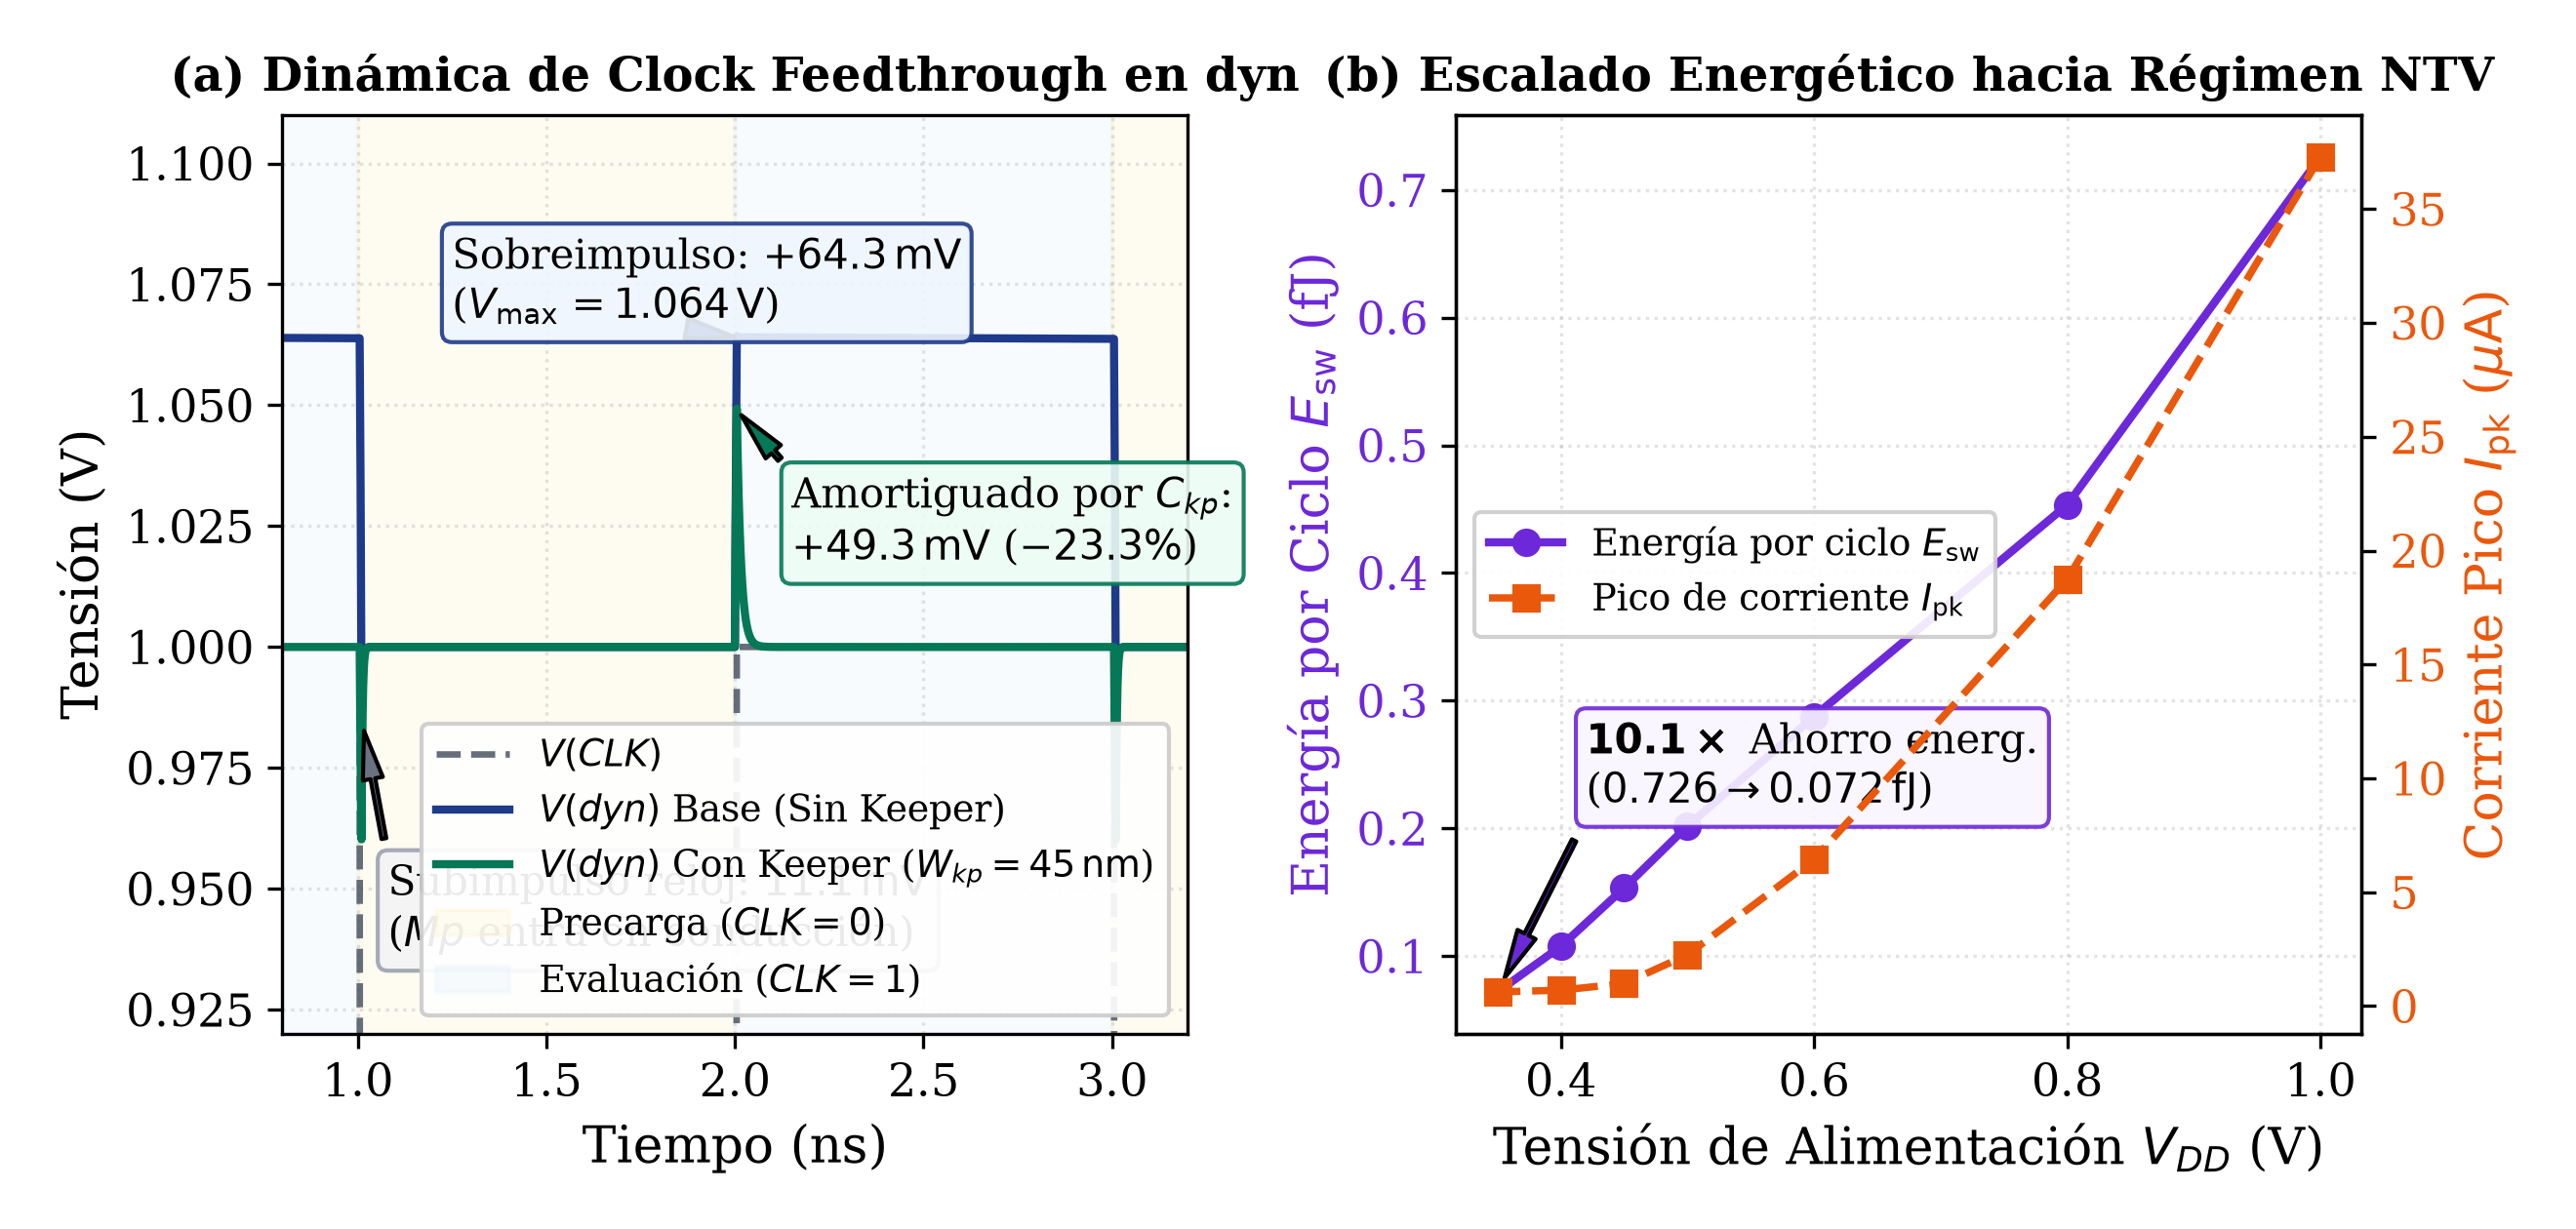
\includegraphics[width=\linewidth,height=3.0cm,keepaspectratio]{figuras/fig1_act5_feedthrough_energia.png}
    \caption[Clock feedthrough y escalado de energía]{Caracterización en PTM 45\,nm HP: (a) Feedthrough en $dyn$ con y sin keeper; (b) Escalado de $I_{\text{pk}}$ y energía dinámica $E_{\text{sw}}$ vs $V_{DD}$.}
    \label{fig:feedthrough_energia}
  \end{minipage}\hfill
  \begin{minipage}[t]{0.485\textwidth}
    \centering
    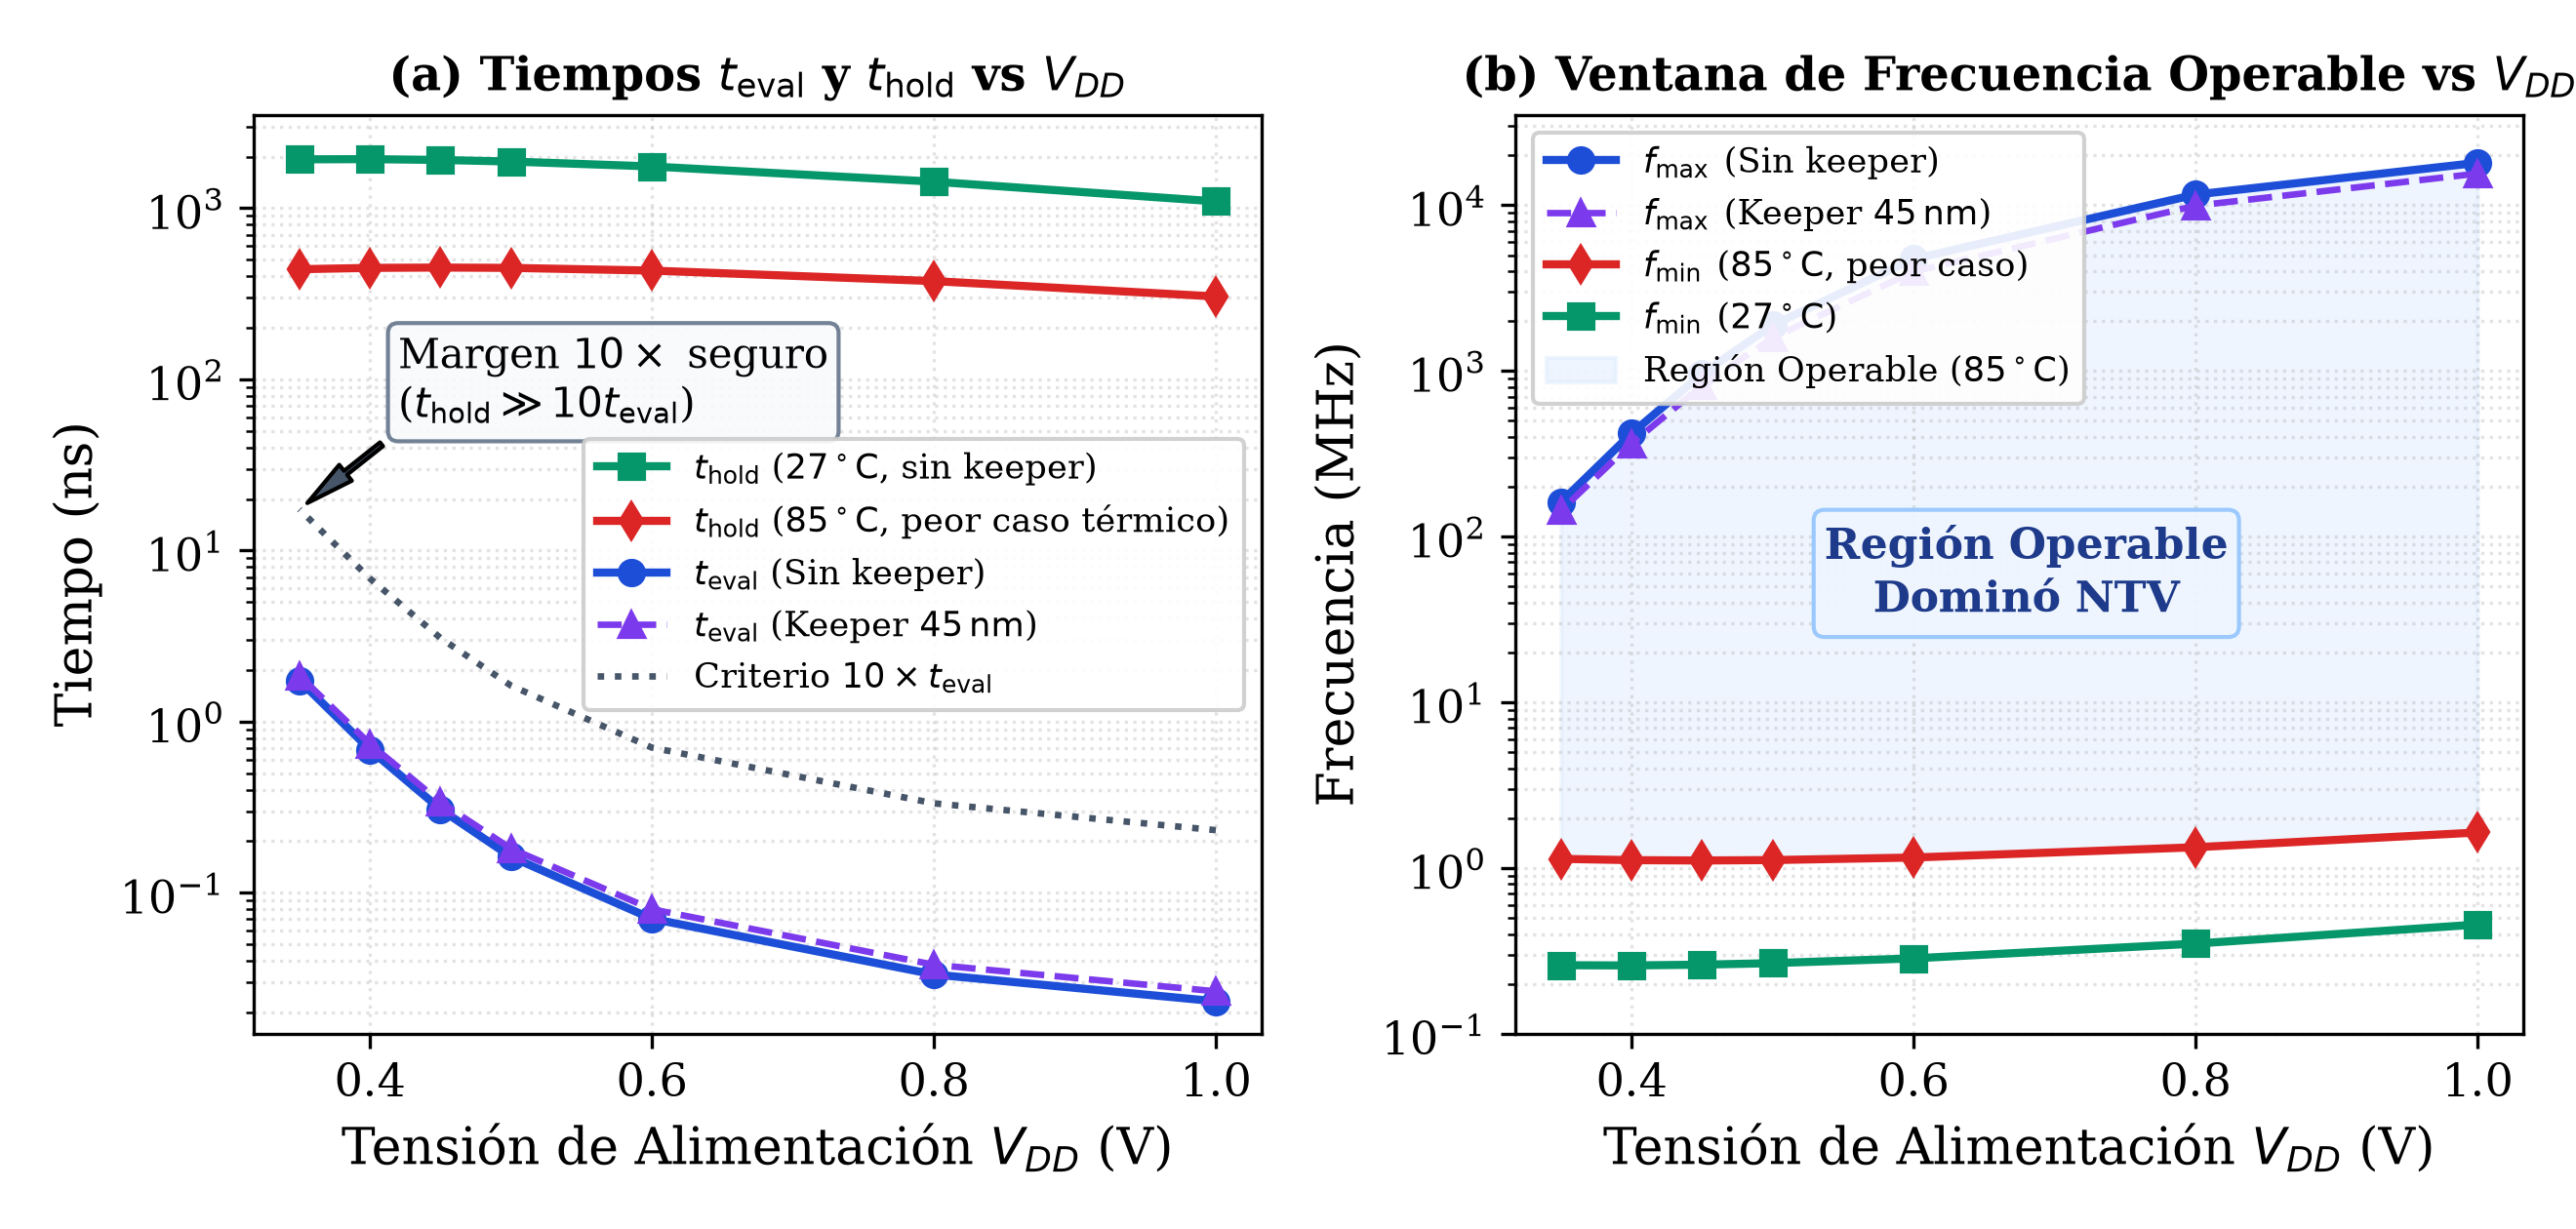
\includegraphics[width=\linewidth,height=3.0cm,keepaspectratio]{figuras/fig2_act5_ventana_frecuencia_ntv.png}
    \caption[Ventana de frecuencia operable NTV]{Frecuencia en PTM 45\,nm HP: (a) $t_{\text{eval}}$ vs $t_{\text{hold}}$ a $27^\circ\text{C}$ y $85^\circ\text{C}$; (b) Ventana operable $[f_{\min}, f_{\max}]$ en MHz reales.}
    \label{fig:ventana_ntv}
  \end{minipage}
\end{figure}

\subsection{Ventana de Frecuencia Operable \texorpdfstring{$[f_{\min}, f_{\max}]$}{[fmin, fmax]} y Operación en Régimen NTV}
La viabilidad operativa está acotada por dos cotas físicas: una frecuencia máxima $f_{\max} \approx 1/(2 \cdot t_{\text{pd}})$, derivada del retardo de la etapa completa ($t_{\text{pd}} = t_{\text{eval}} + t_{pLH,\text{inv}}$), y una frecuencia mínima $f_{\min} \approx 1/(2 \cdot t_{\text{hold}})$, impuesta por la fuga estática. Se precisa que $f_{\max}$ es una \textbf{cota analítica superior estimada desde el retardo transitorio}, no una oscilación periódica sostenida.

\begin{itemize}[leftmargin=1.4em,itemsep=0.01em]
  \item \textbf{Cota Superior ($f_{\max}$) y Penalización por Contención en NTV:} A $V_{DD}=1.0\,\text{V}$, la etapa dominó conmuta en $t_{\text{pd}} = 27.72\,\text{ps} \implies f_{\max} = \mathbf{18.035\,\text{GHz}}$ ($t_{\text{eval}}=33.56\,\text{ps}$ en celda aislada sin carga de inversor). A $0.35\,\text{V}$, la pérdida de sobremarcha eleva el retardo a $t_{\text{pd}} = 3087.20\,\text{ps} \implies f_{\max} = \mathbf{161.96\,\text{MHz}}$. La contención de un keeper de $45\,\text{nm}$ incrementa $t_{\text{pd}}$ a $32.20\,\text{ps}$ ($15.53\,\text{GHz}$) en $1.0\,\text{V}$ y a $3468.80\,\text{ps}$ ($144.14\,\text{MHz}$) en $0.35\,\text{V}$ ($+12.4\%$).
  \item \textbf{Cota Inferior ($f_{\min}$) e Impacto Térmico:} En $1.0\,\text{V}$, la fuga subumbral ($27^\circ\text{C}$) fija $t_{\text{hold}} = 1.096\,\mu\text{s} \implies f_{\min} = \mathbf{456.21\,\text{kHz}}$ ($447.23\,\text{kHz}$ en ensayo de referencia previo). A $85^\circ\text{C}$, las fugas térmicas contraen la retención a $t_{\text{hold}} = 0.305\,\mu\text{s}$ ($1.0\,\text{V}$) y $0.440\,\mu\text{s}$ ($0.35\,\text{V}$), elevando $f_{\min}$ a $\mathbf{1.639\,\text{MHz}}$ y $\mathbf{1.136\,\text{MHz}}$ (aceleración de $\sim 3.6\times$).
  \item \textbf{Criterio de Seguridad $t_{\text{hold}} \ge 10 \cdot t_{\text{eval}}$:} En todo el rango caracterizado ($V_{DD} \in [0.35, 1.00]\,\text{V}$), la ventana operable $[f_{\min}, f_{\max}]$ \textbf{permanece abierta} (Figura~\ref{fig:ventana_ntv}(b)), con $f_{\max}/f_{\min} = 142\times$ y $t_{\text{hold}}/t_{\text{eval}} = 1\,109 \gg 10$ en el peor caso ($0.35\,\text{V}$, $85^\circ\text{C}$).
  \item \textbf{Precisión Metodológica sobre $0.25\,\text{V}$ y $0.30\,\text{V}$:} Las pruebas de retención confirmaron retenciones válidas a $0.30\,\text{V}$ ($1.89\,\mu\text{s}$) y $0.25\,\text{V}$ ($1.80\,\mu\text{s}$), pero al no evaluarse retardo activo ni energía por debajo de $0.35\,\text{V}$, la ventana formal completa se delimita rigurosamente en $[0.35, 1.00]\,\text{V}$.
  \item \textbf{Retención con Keeper:} Con keeper ($W_{kp} \in \{45, 90\}\,\text{nm}$), el equilibrio $I_{kp} \approx I_{\text{sub}}$ mantiene caída $<0.6\,\text{mV}$ en $15\,\mu\text{s}$, fijando una cota inferior observada $t_{\text{hold}} > 15\,\mu\text{s} \implies f_{\min} < \mathbf{33.3\,\text{kHz}}$.
\end{itemize}

\begin{table}[htbp]
\centering
\fontsize{7.5pt}{8.8pt}\selectfont
\caption[Consolidación de métricas de conmutación, retención y energía en NTV]{Consolidación experimental en régimen NTV (PTM 45\,nm HP, $C_L=0.5\,\text{fF}$): retardo de evaluación, frecuencias operables estimadas ($f_{\max}$ calculada desde $t_{\text{pd}}$) y escalado de energía.}
\label{tab:ntv_resumen}
\begin{tabularx}{\linewidth}{@{}>{\centering\arraybackslash}p{1.0cm} >{\centering\arraybackslash}p{1.2cm} >{\centering\arraybackslash}p{1.2cm} >{\centering\arraybackslash}p{1.3cm} >{\centering\arraybackslash}p{1.4cm} >{\centering\arraybackslash}p{1.4cm} >{\centering\arraybackslash}p{1.3cm} >{\centering\arraybackslash}p{1.3cm} >{\RaggedRight\arraybackslash}X@{}}
\toprule
\textbf{$V_{DD}$} & \textbf{$t_{\text{eval}}$} & \textbf{$t_{\text{pd}}$} & \textbf{$f_{\max}$ Act5} & \textbf{$t_{\text{hold}}$ 27°C} & \textbf{$f_{\min}$ 27°C} & \textbf{$f_{\min}$ 85°C} & \textbf{Energía} & \textbf{Diagnóstico y Margen} \\
\textbf{(V)} & \textbf{(ps)} & \textbf{(ps)} & \textbf{(GHz)} & \textbf{($\mu\text{s}$)} & \textbf{(kHz)} & \textbf{(MHz)} & \textbf{($E_{\text{sw}}$, fJ)} & \textbf{de Seguridad ($t_{\text{hold}}/t_{\text{eval}}$)} \\
\midrule
$1.00$ & $23.21$  & $27.72$   & $\mathbf{18.035}$ & $1.096$ & $456.2$ & $1.64$ & $0.7259$ & Nominal HP ($47\,200 \gg 10$). \\
$0.80$ & $33.31$  & $43.11$   & $\mathbf{11.599}$ & $1.429$ & $349.9$ & $1.33$ & $0.4533$ & Retardo $+55\%$, energía $-38\%$. \\
$0.60$ & $70.48$  & $105.40$  & $\mathbf{4.744}$  & $1.754$ & $285.0$ & $1.16$ & $0.2876$ & Balance óptimo energía-retardo. \\
$0.50$ & $162.34$ & $264.52$  & $\mathbf{1.890}$  & $1.874$ & $266.7$ & $1.12$ & $0.2018$ & Régimen NTV ($11\,543 \gg 10$). \\
$0.45$ & $308.17$ & $520.47$  & $\mathbf{0.961}$  & $1.914$ & $261.2$ & $1.11$ & $0.1533$ & Transición a subumbral. \\
$0.40$ & $686.10$ & $1191.33$ & $\mathbf{0.420}$  & $1.935$ & $258.4$ & $1.12$ & $0.1076$ & $f_{\max} = 420\,\text{MHz} \gg f_{\min}$. \\
$0.35$ & $1739.95$& $3087.20$ & $\mathbf{0.162}$  & $1.930$ & $259.1$ & $1.14$ & $0.0719$ & Subumbral: $E_{\text{sw}}$ $-90.1\%$ ($1109 \gg 10$). \\
\bottomrule
\end{tabularx}
\end{table}

\subsection{Comparativa Subumbral a \texorpdfstring{$V_{DD} = 0.50\,\text{V}$}{VDD = 0.50 V}: 45nm HP vs 45nm LP y Energía}
Bajo polarización idéntica a $V_{DD} = 0.50\,\text{V}$ ($T=27^\circ\text{C}$, $C_L=0.5\,\text{fF}$), se contrastó el desempeño subumbral entre las variantes de alto rendimiento (HP) y bajo consumo (LP):

\begin{itemize}[leftmargin=1.4em,itemsep=0.01em]
  \item \textbf{Corrientes y Selectividad:} En 45nm LP, el mayor espesor de óxido (en NMOS: $t_{oxe} = 1.80\,\text{nm}$, $t_{oxp}=1.50\,\text{nm}$, $d_{tox}=0.30\,\text{nm}$ vs $1.25\,\text{nm}$, $1.00\,\text{nm}$, $0.25\,\text{nm}$ en HP; en PMOS $t_{oxe}=1.82\,\text{nm}$ vs $1.30\,\text{nm}$) y $V_{thn} = 0.623\,\text{V} > V_{DD}$ reducen la fuga $I_{\text{off}}$ a $\mathbf{0.671\,\text{pA}}$ vs $\mathbf{125.05\,\text{pA}}$ en HP ($\mathbf{186.4\times}$ menor fuga). La selectividad $I_{\text{on}}/I_{\text{off}}$ asciende a $146\,950$ ($3.75\times$ superior a HP).
  \item \textbf{Compromiso de Retardo:} La menor corriente activa en LP ($98.6\,\text{nA}$ vs $4.898\,\mu\text{A}$) incrementa el retardo a $t_{\text{eval,LP}} = \mathbf{8488.41\,\text{ps}}$ frente a $\mathbf{161.57\,\text{ps}}$ en HP ($\mathbf{52.54\times}$ más lento; $8647.61\,\text{ps}$ en ensayo de celda aislada, apenas $1.8\%$ de discrepancia).
  \item \textbf{Escalado de Energía por Ciclo ($E_{\text{sw}}$):} La integración de corriente en $10\,\text{ns}$ demuestra una reducción de $E_{\text{sw}} = \mathbf{0.7259\,\text{fJ}}$ a $1.0\,\text{V}$ ($I_{\text{pk}} = 37.29\,\mu\text{A}$) hasta $\mathbf{0.0719\,\text{fJ}}$ a $0.35\,\text{V}$ ($I_{\text{pk}} = 0.62\,\mu\text{A}$), logrando un ahorro energético del $\mathbf{90.1\%}$ ($\mathbf{10.1\times}$ de reducción, Tabla~\ref{tab:ntv_resumen}).
\end{itemize}

\subsection{Conclusiones de la Actividad 5}
\begin{enumerate}[leftmargin=1.4em,itemsep=0.01em]
  \item \textbf{Amortiguamiento del Feedthrough:} El sobreimpulso por acoplamiento capacitivo ($+64.31\,\text{mV}$) queda acotado pasivamente por el diodo $D_{DB}$ y se atenúa un $23.3\%$ ($+49.31\,\text{mV}$) por la capacitancia intrínseca añadida por el keeper PMOS.
  \item \textbf{Viabilidad de Lógica Dominó en NTV:} La lógica dominó es viable en tensiones reducidas ($V_{DD} \ge 0.35\,\text{V}$) preservando una ventana operable de $[1.14\,\text{MHz}, 161.96\,\text{MHz}]$ a $85^\circ\text{C}$ con holgura $t_{\text{hold}} \gg 10 \cdot t_{\text{eval}}$. Su coste respecto a la lógica estática radica en una mayor sensibilidad al ruido y la necesidad imperiosa de un keeper dimensionado para evitar el vaciado subumbral ante detenciones de reloj.
  \item \textbf{Compromiso Tecnológico HP vs LP:} El nodo LP proporciona una selectividad $I_{\text{on}}/I_{\text{off}}$ $3.75\times$ superior con fugas $186\times$ menores, garantizando retención estática sin keeper, pero sufre una severa penalización de velocidad ($52.5\times$ más lenta) que restringe su uso a sistemas de baja frecuencia.
\end{enumerate}
